\newpage
\section{Punto 3}
\textit{Aplicar la técnica de ramificación y poda al problema de la Asignación de Tareas, utilizando la siguiente tabla con los costos correspondientes:
}
\begin{figure}[!htb]
  \centering
  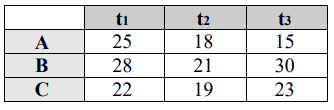
\includegraphics[width=8cm, scale=1]{Images/Punto3/enunciado.png}
  \caption{Tabla de costos}
\end{figure}

Inicialmente se pueden calcular las cotas inferiores y superiores para eliminar posibles casos definiendo un intervalo donde se espera este el resultado, entonces para calcular la cota inferior se tomaran los menores costos de cada fila $A\rightarrow T3 = 15$, $B\rightarrow T2 = 21$, $C\rightarrow T1 = 22$, obteniendo $LB = 15+21+22 = 58$. Luego para la cota superior se puede calcular la sumatoria de la diagonal principal y de la diagonal secundaria y tomar la que de menor resultado, en este caso $DiagonalPrincipal = 25+21+23=69$ y $DiagonalSecundaria = 15+21+22=58$ es decir que $UB = 58$, finalmente se tendrá que el menor resultado estará en el intervalo $[58,58]$ por lo que se deduce que el menor resultado sera 58

Luego se construye un árbol donde a partir de una raíz vacía se van a expandir todas las posibles asignaciones de tareas para A y para cada uno de los nuevos nodos expandidos se calculara su cota inferior nuevamente, luego se expandirá el nodo con menor cota inferior hasta que no queden nodos que puedan expandirse ya que todos los restantes son mayores a la cota inferior del ultimo nodo expandido.

Para el desarrollo de la imagen \ref{fig:poda} a la hora de calcular la cota inferior de cada nodo se obtuvieron los menores costos para cada tarea, es decir se tomo el menor valor de cada columna

\begin{figure}[!htb]
  \centering
  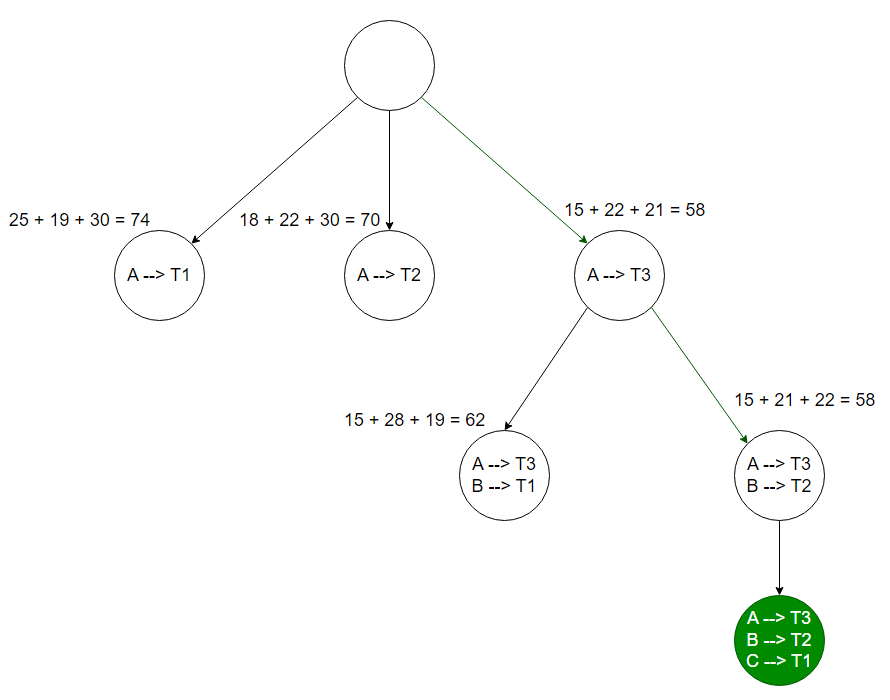
\includegraphics[width=\textwidth, scale=1]{Images/Punto3/Poda.png}
  \caption{Resolución aplicando técnica de ramificación y poda}
  \label{fig:poda}
\end{figure}


